\makeheading{Lecture 11 | 2020-10-19}
\section{ANOVA F Test}
Recall the general linear hypothesis:
$ H_0 $: $ A\symbf{\beta}=\symbf{0} $
vs $ H_A $: $ A\symbf{\beta}\neq \symbf{0} $
where $ A $ gives $ \ell $ constraints.

\[ F\text{ statistic}=
      \frac{(\SS{Res}_A-\SS{Res})/\ell}{\SS{Res}/(n-p-1)}=
      \frac{(\SS{Res}_A-\SS{Res})/\ell}{\hat{\sigma}^2}  \]
compare to $ F(\ell,n-p-1) $.

Special case: overall test of significance

``Are any predictors related to response?''
\begin{itemize}
      \item $ H_0 $: $ \beta_1=\beta_2=\cdots=\beta_p=0 $
      \item $ H_A $: $ \beta_j\neq 0 $ for at least one $ j $
\end{itemize}
\[ A=\begin{bmatrix}
            0      & 1 & 0 & 0      & \cdots & 0 & 0 \\
            0      & 0 & 1 & 0      & \cdots & 0 & 0 \\
            \vdots &   &   & \ddots                  \\
            0      & 0 & 0 & 0      & \cdots & 1 & 0 \\
            0      & 0 & 0 & 0      & \cdots & 0 & 1 \\
      \end{bmatrix}\begin{bmatrix}
            \beta_0     \\
            \beta_1     \\
            \vdots      \\
            \beta_{p-1} \\
            \beta_p
      \end{bmatrix} \]
If $ H_0 $ is true: $ Y_i=\beta_0+\varepsilon_i $
where $ Y_i \sim \N{\beta_0,\sigma^2} $.

Fit reduced model; that is, in this case estimate $ \beta_0 $
using the least squares, minimize $ \sum_{i=1}^{n} (y_i-\beta_0)^2 $,
which can be shown $ \hat{\beta}_0=\bar{y} $. So,
\[ \SS{Res}_A
      =\sum_{i=1}^{n} e_i^2
      =\sum_{i=1}^{n} (y_i-\hat{\mu}_i)^2
      =\sum_{i=1}^{n}(y_i-\bar{y})^2
      =\SS{Total} \]
Then,
\[ F=\frac{(\SS{Total}-\SS{Res})/p}{\SS{Res}/(n-p-1)}
      =\frac{\SS{Reg}/p}{\SS{Res}/(n-p-1)}
      =\frac{\MS{Reg}}{\MS{Res}}
      \leftarrow F\text{ statistic on ANOVA table}    \]
\subsection{R Demo}
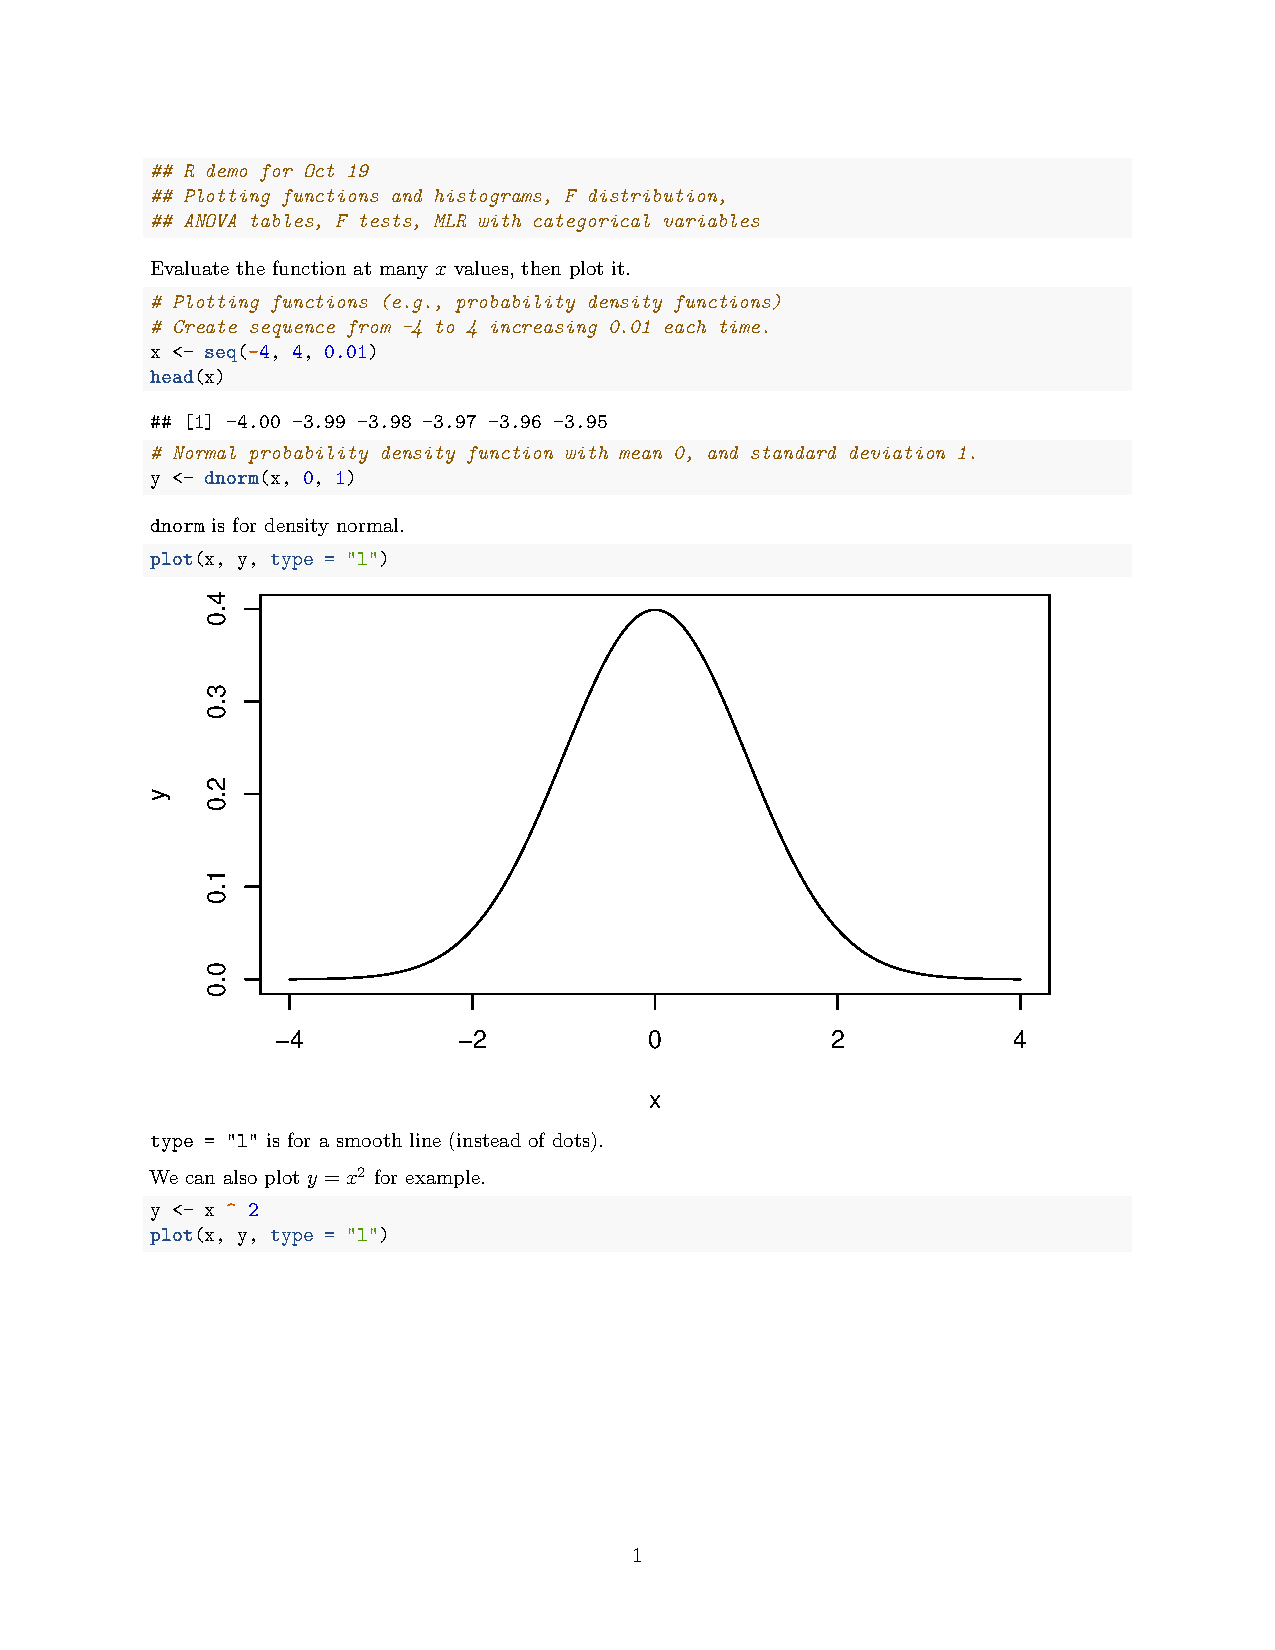
\includepdf[pages=-]{lec_11-demo.pdf}
